\chapter{Recurrent Network Models}
\label{ch:networks}

\textit{Network models ask how connectivity transforms single-neuron responses into collective dynamics. This chapter develops rate equations, eigenmode analysis, and structured recurrence as mechanisms for amplification, selection, and persistent activity.}

% ============================================================
\section{From Spikes to Firing Rates}
\label{sec:spikes-to-rates}
% ============================================================

Everything in this course so far has described individual neurons: their membrane potentials, channel kinetics, and cable properties. But the brain contains billions of neurons operating together. To study networks, we need to shift from tracking individual spikes to tracking \emph{population activity}---the firing rate of groups of neurons.

The simplest version of this transition replaces the detailed spike-generating dynamics with a static input--output function. If the synaptic input current to a neuron varies slowly compared to the membrane time constant, the neuron's firing rate tracks the steady-state $f$--$I$ curve:
%
\begin{equation}
  v(t) = F\bigl(I_s(t)\bigr)
  \label{eq:static-rate}
\end{equation}
%
where $F$ is the activation function---the neuron's $f$--$I$ curve, which maps input current to firing rate. For Type~I neurons, $F$ rises smoothly from zero; for Type~II neurons, it jumps to a nonzero value.

This steady-state approximation works well when inputs change slowly. For fast-varying inputs, the neuron cannot keep up instantaneously: there is a lag between changes in input and changes in firing rate. The Wilson--Cowan model accounts for this by adding a phenomenological time constant:
%
\begin{equation}
  \tau_r \frac{\dd v}{\dd t} = -v + F\bigl(I(t)\bigr)
  \label{eq:wilson-cowan}
\end{equation}
%
The time constant $\tau_r$ is not simply the membrane time constant $\taum$---it depends on input strength, noise, and network context. It represents the lag between changes in input and changes in population firing rate.

% ============================================================
\section{Network Architecture}
\label{sec:network-architecture}
% ============================================================

A network of $N$ firing-rate neurons has a state vector $\vec{v}(t) \in \R^N$ (the firing rates of all neurons) driven by an input vector $\vec{u}(t)$ (external drive). The network is defined by two weight matrices: a \emph{feedforward} matrix $W$ that maps inputs to internal drive, and a \emph{recurrent} matrix $M$ that describes how neurons influence each other.

\begin{keyequation}[General Recurrent Rate Model]
\begin{equation}
  \tau_r\,\dot{\vec{v}} = -\vec{v} + F\bigl(W\vec{u} + M\vec{v}\bigr)
  \label{eq:rate-network}
\end{equation}
\tcblower
$\vec{v}$: firing rate vector, \quad
$\vec{u}$: external input, \quad
$W$: feedforward weights, \quad
$M$: recurrent weights, \quad
$F$: activation function.
\end{keyequation}

\noindent The feedforward term $W\vec{u}$ transforms and filters the input. The recurrent term $M\vec{v}$ feeds the network's own activity back into itself. The interplay between feedforward drive and recurrent feedback determines the network's computational behavior.

% ============================================================
\section{Linear Recurrent Networks}
\label{sec:linear-networks}
% ============================================================

The simplest case sets $F$ to the identity function, giving a linear system:
%
\begin{equation}
  \tau_r\,\dot{\vec{v}} = -\vec{v} + \vec{h} + M\vec{v}
  \label{eq:linear-network}
\end{equation}
%
where $\vec{h} = W\vec{u}$ is the feedforward drive. Despite its simplicity, this linear model reveals the essential logic of recurrent computation.

\subsection{Eigenmode decomposition}

If $M$ is symmetric (a simplification; real connectivity is not), its eigenvalues $\lambda_\mu$ are real and its eigenvectors $\vec{e}_\mu$ are orthogonal. Expanding the state as $\vec{v}(t) = \sum_\mu c_\mu(t)\,\vec{e}_\mu$, each mode decouples:

\begin{keyequation}[Eigenmode Dynamics]
\begin{equation}
  \tau_r\,\dot{c}_\mu = -(1 - \lambda_\mu)\,c_\mu + \vec{e}_\mu \cdot \vec{h}
  \label{eq:eigenmode}
\end{equation}
\tcblower
$c_\mu(t)$: amplitude of mode $\mu$, \quad
$\lambda_\mu$: eigenvalue of $M$, \quad
$\vec{e}_\mu \cdot \vec{h}$: projection of input onto mode $\mu$.
\end{keyequation}

\noindent Each mode evolves independently as a simple first-order equation. The effective time constant is $\tau_r/(1 - \lambda_\mu)$, and the steady-state amplitude (for stable modes) is $c_\mu(\infty) = (\vec{e}_\mu \cdot \vec{h})/(1 - \lambda_\mu)$.

\subsection{Stability, amplification, and integration}

The eigenvalue $\lambda_\mu$ controls everything about mode $\mu$:

If $\lambda_\mu < 1$, the mode is stable. The input component along $\vec{e}_\mu$ is amplified by a gain factor $1/(1 - \lambda_\mu)$, and the effective time constant is stretched by the same factor. Eigenvalues close to $1$ produce strong amplification and slow dynamics.

If $\lambda_\mu > 1$, the mode is unstable: the corresponding pattern of activity grows exponentially. In a real network, nonlinearities (saturation, rectification) eventually bound the growth, but in the linear model, this represents an explosion.

If $\lambda_\mu = 1$ exactly, the leak and recurrent feedback cancel perfectly, and the mode becomes a \emph{perfect integrator}:
%
\begin{equation}
  c_1(t) = \frac{1}{\tau_r}\int_0^t \vec{e}_1 \cdot \vec{h}(t')\;\dd t'
  \label{eq:perfect-integrator}
\end{equation}
%
The network accumulates input along $\vec{e}_1$ without decay---a form of persistent activity or working memory. But this requires $\lambda_1 = 1$ with infinite precision. If $\lambda_1 = 0.99$, the memory leaks away; if $\lambda_1 = 1.01$, activity explodes. This \emph{fine-tuning problem}\index{fine-tuning problem} is a central challenge for linear models of persistent activity.

\subsection{Selective amplification}

When one eigenvalue is close to $1$ and the others are small, the network strongly amplifies the input component that matches the corresponding eigenvector, while other components are only weakly amplified or suppressed. The network acts as a ``matched filter''---it selectively extracts the pattern it is tuned to represent.

% ============================================================
\section{The Ring Network}
\label{sec:ring-network}
% ============================================================

The ring network\index{ring network} is a concrete example that ties together selective amplification, pattern formation, and biological function. It models neurons arranged in a circle, each with a preferred direction (as in the head-direction system\index{head-direction cells} of the fly or the mammalian thalamus).

The recurrent connectivity depends on the angular difference between neurons:
%
\begin{equation}
  M(\theta, \theta') \propto \cos(\theta - \theta')
  \label{eq:ring-connectivity}
\end{equation}
%
Nearby neurons (similar preferred directions) excite each other; distant neurons inhibit each other. This ``Mexican hat'' connectivity profile has a clean eigenstructure: the eigenvectors are Fourier modes (cosines and sines), and the fundamental mode (a single bump) has the largest eigenvalue.

If the fundamental eigenvalue is set near $1$ while higher harmonics have small eigenvalues, the network selectively amplifies broad, smooth patterns of activity. A noisy input with multiple peaks is cleaned up: the network sustains a single bump of activity centered on the most strongly driven direction. This bump represents the animal's current heading.

\subsection{Persistent activity and path integration}

In darkness, with no sensory input, the bump persists---a memory of the last known heading. This is the ring attractor\index{ring attractor} functioning as a working memory for a continuous variable. The bump can be shifted by vestibular or motor signals (velocity inputs), implementing \emph{path integration}: updating the heading estimate based on self-motion.

Experimental recordings from the fly's ellipsoid body confirm this picture: calcium imaging reveals a bump of activity that rotates with the fly's heading, persists in darkness, and drifts slowly without visual landmarks (confirming that the system is an imperfect integrator).

Comparable head-direction populations in rodents show related behavior: internally generated heading signals are stable over short intervals but accumulate drift without external reference cues. Visual and landmark input then acts as an error-correction channel, pulling the bump back toward veridical heading.

This drift-correction interplay is computationally central. Pure path integration accumulates error; pure sensory tracking fails when cues are absent. The ring network provides a principled fusion architecture where recurrent dynamics maintain memory and sensory input periodically re-anchors it.

% ============================================================
\section{Nonlinear Networks: Rectification and Winner-Take-All}
\label{sec:nonlinear-networks}
% ============================================================

Linear networks have a serious problem: firing rates can be negative, which is unphysical. Adding a rectifying nonlinearity---$F(x) = [x]_+ = \max(0, x)$---fixes this and fundamentally changes the network's behavior.

Rectification turns amplification into \emph{selection}\index{winner-take-all}. In a linear network, all modes are amplified (some more than others). With rectification, the strongly amplified mode drives competing neurons' rates to zero, and only the winning pattern survives. This is winner-take-all dynamics: the network selects the single input direction that best matches its recurrent structure and suppresses everything else.

In the ring network, rectification sharpens the activity bump and creates a robust attractor. The bump can sit at any angle on the ring---the set of all possible bump positions forms a \emph{ring attractor}\index{ring attractor}. Unlike the fine-tuned linear integrator, the nonlinear ring attractor sustains activity without requiring $\lambda = 1$ exactly. Nonlinearity provides the robustness that linear models lack.

The feedforward weights $W$ determine the initial response to a sensory input (its ``shape''), while the recurrent weights $M$ govern what happens afterward: amplification, selection, and sustained memory through feedback.

\begin{figure}[h]
\centering
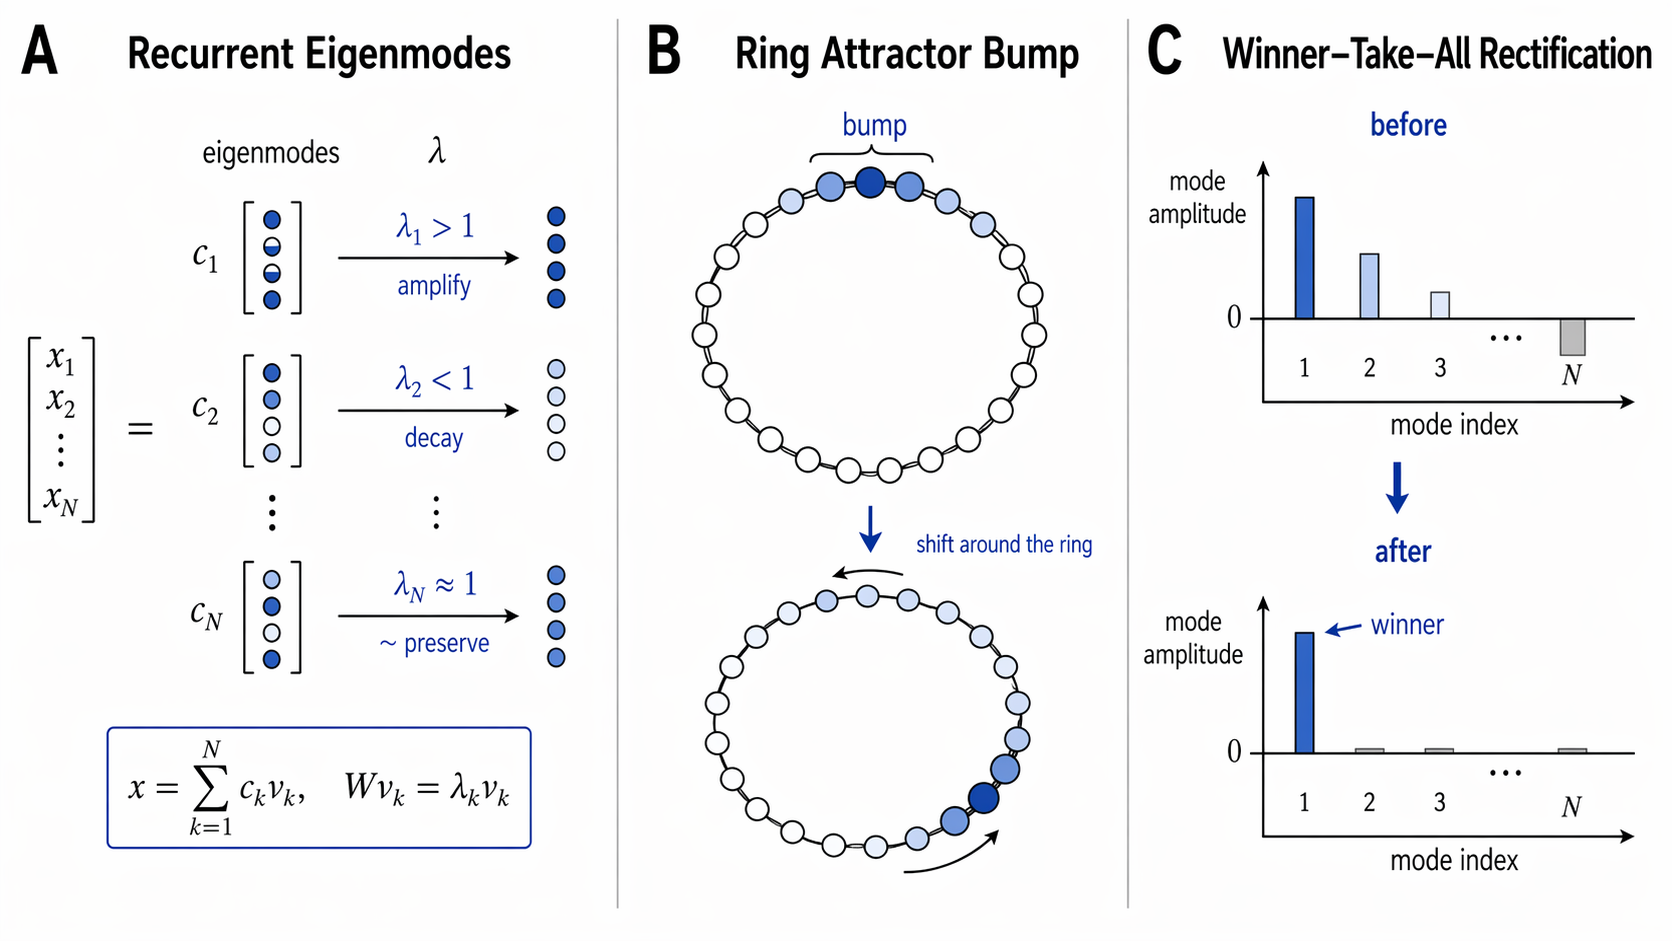
\includegraphics[width=\textwidth]{figures/mns-network-modes-attractors.png}
\caption{Recurrent network computations. Eigenmodes decompose linear amplification, ring attractors store a continuous bump state, and rectification turns graded amplification into winner-take-all selection.}
\label{fig:network-modes-attractors}
\end{figure}

\subsection{Beyond winner-take-all: gain modulation, associative memory, and oscillations}

Rectified recurrent networks support more than input selection. Three extensions are especially useful:
\begin{enumerate}
  \item \textbf{Gain modulation}: recurrent context can scale response amplitude without changing preferred feature, implementing multiplicative-like computations used in sensorimotor transformations.
  \item \textbf{Associative memory}: with structured recurrent weights (e.g., Hebbian imprinting of patterns), activity can converge to stored attractors, enabling pattern completion from partial cues.
  \item \textbf{Oscillatory regimes}: with suitable excitation--inhibition balance and delays, recurrent networks can generate rhythmic population activity rather than fixed-point attractors.
\end{enumerate}

These behaviors are not separate model classes; they are different operating regimes of the same recurrent architecture under different nonlinearities and connectivity structure.

Computationally, this is why recurrent models are versatile: the same circuit motif can denoise, select, integrate, memorize, and synchronize depending on parameter regime and input context.


\begin{chaptersummary}

\begin{center}
\renewcommand{\arraystretch}{1.6}
\begin{tabularx}{\textwidth}{@{}l X X@{}}
  \toprule
  \textbf{Concept} & \textbf{Equation} & \textbf{Key Insight} \\
  \midrule
  Rate model &
  $\tau_r\dot{\vec{v}} = -\vec{v} + F(W\vec{u} + M\vec{v})$ &
  Feedforward drive + recurrent feedback \\
  %
  Eigenmode &
  $\tau_r\dot{c}_\mu = -(1 - \lambda_\mu)c_\mu + \vec{e}_\mu \cdot \vec{h}$ &
  Each mode evolves independently \\
  %
  Amplification &
  $\displaystyle\text{Gain} = \frac{1}{1 - \lambda_\mu}$ &
  $\lambda \to 1$: strong amplification, slow dynamics \\
  %
  Perfect integrator &
  $\lambda = 1$: no decay &
  Working memory, but requires fine-tuning \\
  %
  Ring connectivity &
  $M \propto \cos(\theta - \theta')$ &
  Head-direction bump, ring attractor \\
  %
  Rectification &
  $F(x) = \max(0, x)$ &
  Selection, winner-take-all, robust attractors \\
  %
  Drift-corrected path integration &
  Internal integration + landmark anchoring &
  Persistent memory with external error correction \\
  %
  Nonlinear recurrent extensions &
  Gain modulation / attractor memory / oscillations &
  One architecture, multiple computational regimes \\
  \bottomrule
\end{tabularx}
\end{center}

\end{chaptersummary}

\begin{conceptquestions}
  \item The transition from spikes to rates involves replacing the detailed spike dynamics with a static $f$--$I$ curve. Under what conditions is this approximation valid? When does it break down?

  \item The Wilson--Cowan equation $\tau_r \dot{v} = -v + F(I)$ introduces a time constant $\tau_r$ that is not simply the membrane time constant. What determines $\tau_r$, and why is it generally faster than $\taum$?

  \item In a linear recurrent network, why does an eigenvalue close to $1$ produce both strong amplification and slow dynamics? What is the connection between these two effects?

  \item For a linear network with eigenvalues $\lambda_1 = 0.95$, $\lambda_2 = 0.5$, $\lambda_3 = 0.1$, compute the gain and effective time constant for each mode. Which mode dominates the response?

  \item The ``fine-tuning problem'' says that $\lambda = 1$ is required for perfect integration but is biologically unrealistic. Why is exact fine-tuning unrealistic? What happens to the ``memory'' if $\lambda = 0.99$ versus $\lambda = 1.01$?

  \item A linear recurrent network with one eigenvalue near $1$ and all others small acts as a ``matched filter.'' What does it filter for, and how does the eigenvector structure determine this selectivity?

  \item Explain how the ring network implements a head-direction system. What does the ``bump'' of activity represent, and how is it maintained and updated?

  \item The ring network has connectivity $M(\theta, \theta') \propto \cos(\theta - \theta')$. Why do the eigenvectors of this connectivity matrix correspond to Fourier modes? Which mode has the largest eigenvalue?

  \item In darkness, the head-direction bump persists but drifts slowly. What does this drift tell you about how close the network's eigenvalue is to $1$? How could the brain correct for this drift?

  \item How does nonlinearity (rectification) solve the fine-tuning problem in the ring network? Why does a rectified bump attractor not require $\lambda = 1$ exactly?

  \item Compare the roles of the feedforward matrix $W$ and the recurrent matrix $M$. Which determines the initial response to a stimulus, and which determines the long-term dynamics? Give an example where each dominates.

  \item Winner-take-all dynamics emerge from the combination of recurrent excitation and rectification. Explain the mechanism: why does the strongest input suppress all others?

  \item A ring attractor can store a continuous variable (like heading angle). How is this different from a discrete attractor network that stores one of a finite number of patterns? What biological computations might require each type?

  \item Why is path integration alone insufficient for long timescales? How do sensory landmarks correct the drift of a recurrent bump representation?

  \item Give one mechanism by which the same recurrent network could move from winner-take-all behavior to oscillatory behavior.

  \item The eigenmode decomposition assumes $M$ is symmetric. Real neural connectivity is typically asymmetric ($M_{ij} \neq M_{ji}$). What qualitatively new phenomena can asymmetric connectivity produce that symmetric connectivity cannot?
\end{conceptquestions}
